%%%%%%%%%%%%%%%%%%%%%%%%%%%%%%%%%%%%%%%%%%%%%%%%%%%%%%%%%%%%%%%%%%%%%
%
% Axel Fahy & Höhn Rudolf
% Automn Semester MSE
% IV
%
%%%%%%%%%%%%%%%%%%%%%%%%%%%%%%%%%%%%%%%%%%%%%%%%%%%%%%%%%%%%%%%%%%%%%%

%----------------------------------------------------------------------------------------
%   PACKAGES AND THEMES
%----------------------------------------------------------------------------------------
\documentclass{beamer}
\usepackage[utf8]{inputenc}
%\usepackage[french]{babel}
\usepackage[T1]{fontenc}
\usepackage{lmodern}
\usepackage{amsmath}
\usepackage{amsfonts}
\usepackage{amssymb}
\usepackage{graphicx}
\usepackage{xcolor}

%\usepackage{pgfpages}
%\setbeameroption{show notes on second screen}    % To show notes (on second screen)

% Bullet color depending on environment
\newenvironment{actifenv}{\only{\setbeamercolor{local structure}{fg=cyan}}}{}

\mode<presentation> {

% The Beamer class comes with a number of default slide themes
% which change the colors and layouts of slides. Below this is a list
% of all the themes, uncomment each in turn to see what they look like.

%\usetheme{default}
%\usetheme{AnnArbor}
%\usetheme{Antibes}
%\usetheme{Bergen}
%\usetheme{Berkeley}
%\usetheme{Berlin}
%\usetheme{Boadilla}
%\usetheme{CambridgeUS}
%\usetheme{Copenhagen}
%\usetheme{Darmstadt}
%\usetheme{Dresden}
\usetheme{Frankfurt}
%\usetheme{Goettingen}
%\usetheme{Hannover}
%\usetheme{Ilmenau}
%\usetheme{JuanLesPins}
%\usetheme{Luebeck}
%\usetheme{Madrid}
%\usetheme{Malmoe}
%\usetheme{Marburg}
%\usetheme{Montpellier}
%\usetheme{PaloAlto}
%\usetheme{Pittsburgh}
%\usetheme{Rochester}
%\usetheme{Singapore}
%\usetheme{Szeged}
%\usetheme{Warsaw}

% As well as themes, the Beamer class has a number of color themes
% for any slide theme. Uncomment each of these in turn to see how it
% changes the colors of your current slide theme.

%\usecolortheme{albatross}
%\usecolortheme{beaver}
%\usecolortheme{beetle}
%\usecolortheme{crane}
%\usecolortheme{dolphin}
%\usecolortheme{dove}
%\usecolortheme{fly}
\usecolortheme{lily}
%\usecolortheme{orchid}
%\usecolortheme{rose}
%\usecolortheme{seagull}
%\usecolortheme{seahorse}
%\usecolortheme{whale}
%\usecolortheme{wolverine}

%\setbeamertemplate{footline} % To remove the footer line in all slides uncomment this line
%\setbeamertemplate{footline}[page number] % To replace the footer line in all slides with a simple slide count uncomment this line

%\setbeamertemplate{navigation symbols}{} % To remove the navigation symbols from the bottom of all slides uncomment this line
}

%\setbeamercovered{transparent}
\setbeamertemplate{navigation symbols}{}
\setbeamertemplate{footline}[frame number]
\useinnertheme{rectangles} % Rectangle bullet points instead of circle ones

%%%%% CONF HYPERREF PACKAGE
\hypersetup{colorlinks=true}

% Show the circle in each section without having subsections
\usepackage{remreset}
\makeatletter
\@removefromreset{subsection}{section}
\makeatother
\setcounter{subsection}{1}

%----------------------------------------------------------------------------------------
%   TITLE PAGE
%----------------------------------------------------------------------------------------

\title{Stocks Trooper}
\author{Axel Fahy \& Rudolf Höhn}
\institute{Information Visualization\\MSE\\\href{https://github.com/rudy2707/Stockstrooper}{GitHub repository}}
%\logo{\includegraphics[width=2cm,height=2cm,keepaspectratio]{logos/logo_hepia_black.png}}
\logo{
    \makebox[0.95\paperwidth]{
        
\includegraphics[scale=0.03]{Figures/st-blue.png}
        % 
\includegraphics[width=2cm,keepaspectratio]{Figures/st-blue.png}
        \hfill
        
\includegraphics[scale=0.25]{Figures/mse-logo.jpg}
    }
}
\date{23.12.2016}
%\subject{}
\begin{document}

%----------------------------------------------------------------------------------------
%   PRESENTATION SLIDES
%----------------------------------------------------------------------------------------

\begin{frame}
\titlepage
\end{frame}


% \begin{frame}
% \tableofcontents
% \end{frame}
%


%----------------------------------------------------------------------------------------
\section{Introduction}
%------------------------------------------------

\begin{frame}{Aim of the project}
    \begin{itemize}
        \item Understand the evolution of an index' price
        \item Mental model between the events occured and the news published around that day
        \item Project for financial analysts and other financial actors
    \end{itemize}
\end{frame}

%------------------------------------------------

\begin{frame}{Source of the data}
    \begin{itemize}
        \item Yahoo Finance for the stocks values
        \item New York Times API for the news
    \end{itemize}
\end{frame}

%------------------------------------------------

\begin{frame}{Technology used}
    \begin{center}
        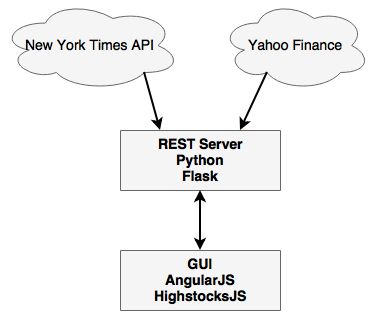
\includegraphics[scale=0.5]{Figures/st-system-architecture.png}
    \end{center}
\end{frame}


%----------------------------------------------------------------------------------------
\section{IV aspects}
\begin{frame}{Demo}
\end{frame}

%----------------------------------------------------------------------------------------
\section{Conclusion}
\begin{frame}{Tools critic}
    \begin{itemize}
        \item AngularJS directive for HighstocksJS not optimal at all
        \item Yahoo Finance API is too slow
        \item New York Times API does not provide enough articles and the links are broken
    \end{itemize}
\end{frame}

\begin{frame}{Project status}
    \begin{itemize}
        \item Needs more test and mostly UX test with the end-users
        \item Flags are not dynamic
    \end{itemize}
\end{frame}

\begin{frame}{Future work}
    \begin{itemize}
        \item Flags could be clickable
        \item Historic of past search
        \item Multiple data sources for the news
        \item Creation of a user profile allowing to change the default parameters
    \end{itemize}
\end{frame}

%----------------------------------------------------------------------------------------
\end{document}
